\chapter[Ferramenta]{Ferramenta e-TAPE}
\label{cap:cap3}
Este trabalho teve como proposta o desenvolvimento de uma aplicação web, chamada e-TAPE, cujo o objetivo consiste em disponibilizar um ambiente para edição colaborativa e evolução da taxonomia TAPE.
Para desenvolver a aplicação foi definida uma metodologia baseada no modelo de ciclo de vida incremental, descrita na seção seguinte.

\section {Metodologia de Desenvolvimento da e-TAPE}
\label{sec:desenvolvimento}
\par
Segundo \citeonline{sommerville2016software}, o modelo incremental é baseado na ideia de se desenvolver uma aplicação inicial a partir do \textit{feedback} de todos os \textit{stakeholders} envolvidos e evoluir a aplicação em versões, até que os requisitos identificados estejam adequadamente atendidos na aplicação. 

\par
Em relação aos atores envolvidos na aplicação, foram identificadas as seguintes classes de usuário:
\begin{itemize}
    \item \textbf{Usuário não cadastrado (visitante)}: consulta as informações disponibilizadas mas não têm permissão para edição. Essa edição inclui propor uma alteração na taxonomia ou classificar novas ferramentas.
    \item \textbf{Usuário cadastrado}: depois de cadastrado, o usuário autenticado pode, além de consultar as informações, propor alterações na taxonomia,  como a criação de uma nova classe, ou incluir/alterar a
    classificação de uma ferramenta. Quando um usuário autenticado propõe evolução da taxonomia, essa proposta deverá ser avaliada por um moderador. Caso o moderador concorde com a modificação,  a taxonomia é modificada. Vale destacar que na elaboração do modelo conceitual dos dados, essa possibilidade foi considerada, as versões antigas da taxonomia permanecem no banco de dados de maneira que seja armazenado
    um histórico. 
    \item \textbf{Usuário moderador}: esse usuário tem as mesmas permissões que o usuário autenticado além de poder alterar a taxonomia e validar as propostas de alterações. 
\end{itemize}

\par
Embora tenham sido identificadas as três classes de usuário descritas, nessa versão inicial, foi considerada somente a classe de usuário visitante.
Contudo, diferente do que foi previsto, o visitante também pode classificar e alterar a classificação de ferramenta. Essa adaptação foi necessária devido ao tempo disponível 
para implementação da e-TAPE e conclusão do trabalho. Apesar disso, o desenvolvimento dessas funcionalidades foi realizada de maneira que essa evolução seja facilmente 
implementada em versões futuras.

\par
Ainda de acordo com \citeonline{sommerville2016software}, cada versão entregue da aplicação deve incorporar novas funcionalidades para melhor atender aos requisitos identificados. Geralmente, as primeiras funcionalidades implementadas são escolhidas pelo grau de importância para o produto final. Esse modelo permite a avaliação da aplicação em versões iniciais de desenvolvimento, para assim saber 
se os requisitos estão sendo entregues. A figura \ref{fig:modelo-incremental} demonstra a abstração do modelo incremental.

\begin{figure}[!ht]
    \centering
    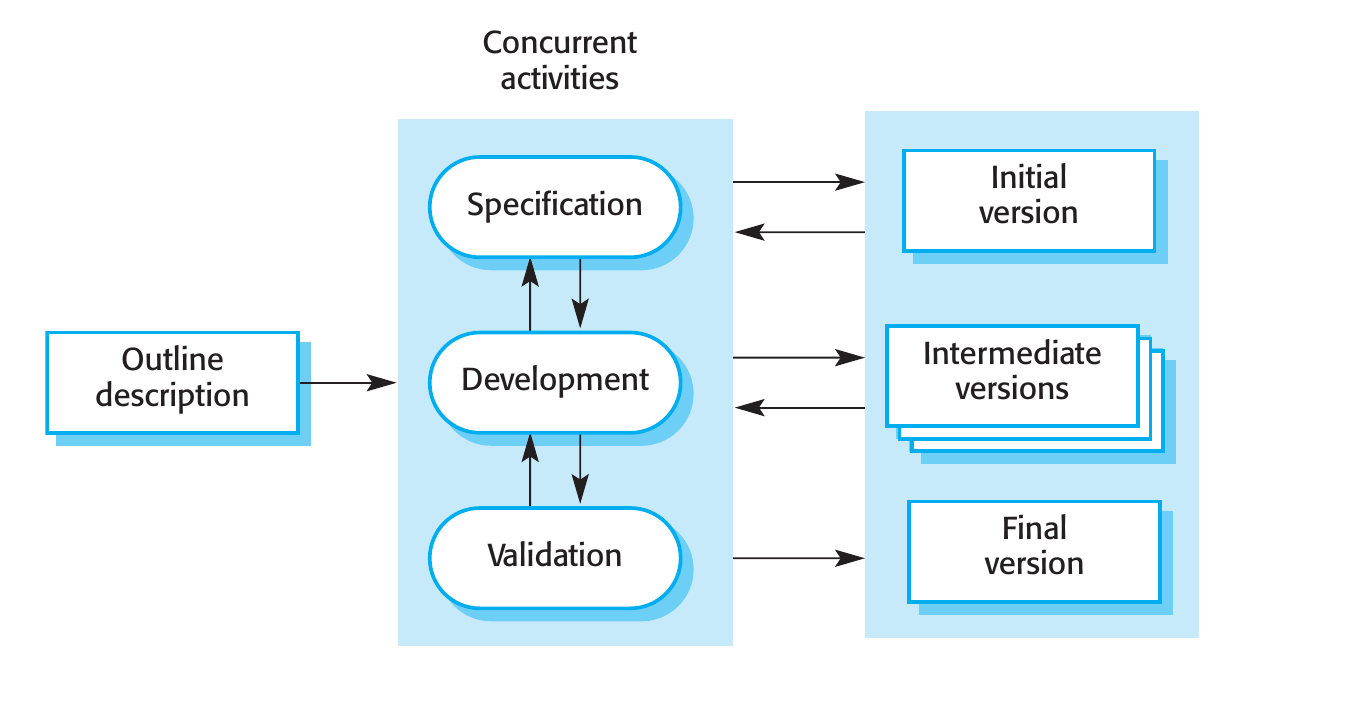
\includegraphics[scale=0.20]{./figuras/modelo_incremental.png}
    \caption{Modelo de desenvolvimento Incremental \citeonline{sommerville2016software}}
    \label{fig:modelo-incremental}
\end{figure}

\par
Para o desenvolvimento da aplicação, foram realizados o levantamento dos requisitos de cliente e a modelagem conceitual dos dados. A lista de requisitos simplificada está no Apêndice \ref{apendice:b}. 
Depois de detalhados os requisitos, foi construído um protótipo que foi validado pelos pesquisadores envolvidos na elaboração da TAPE. A ferramenta e-TAPE está disponível em http://taxonopart.hopto.org:3001.

\par
Ao acessar o endereço da aplicação, o usuário visitante encontra uma breve explicação sobre o contexto do projeto e uma descrição da taxonomia considerando os grupos,
classes e subclasses propostas. É possível obter detalhes, sobre as classes e subclasses, clicando em seus respectivos nomes. 

\par
Ao acessar a página Taxonomia, o usuário visitante começa sua interação ativa com a aplicação.
Foram disponibilizados dois modos de visualização da taxonomia: o e-TAPE 360º e o e-TAPE Árvore, ilustrados, respectivamente,
nas Figuras \ref{fig:e-tape360} e \ref{fig:e-tapeArvore}. Podendo-se alterar entre os modos de visualização ao clique de um botão.

\begin{figure}[!ht]
    \centering
    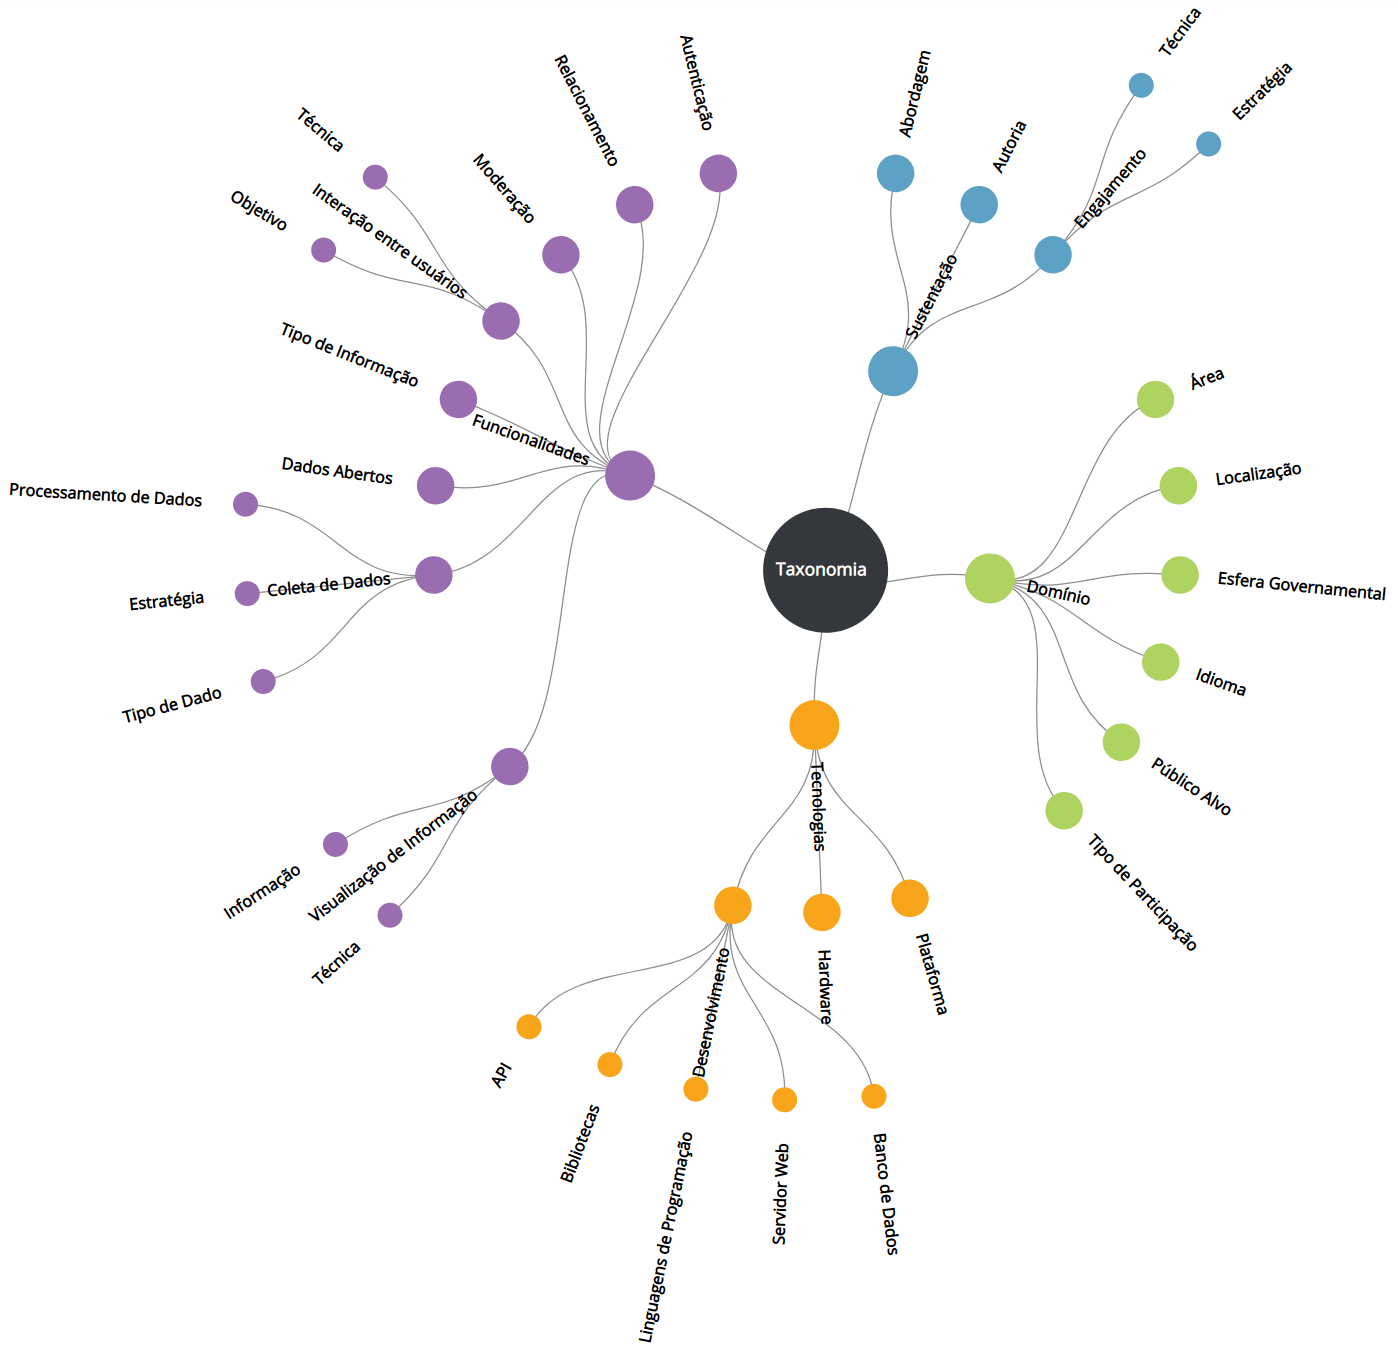
\includegraphics[scale=0.20]{./figuras/taxonomia-cropped.png}
    \caption{e-TAPE 360º}
    \label{fig:e-tape360}
\end{figure}

\begin{figure}[!ht]
    \centering
    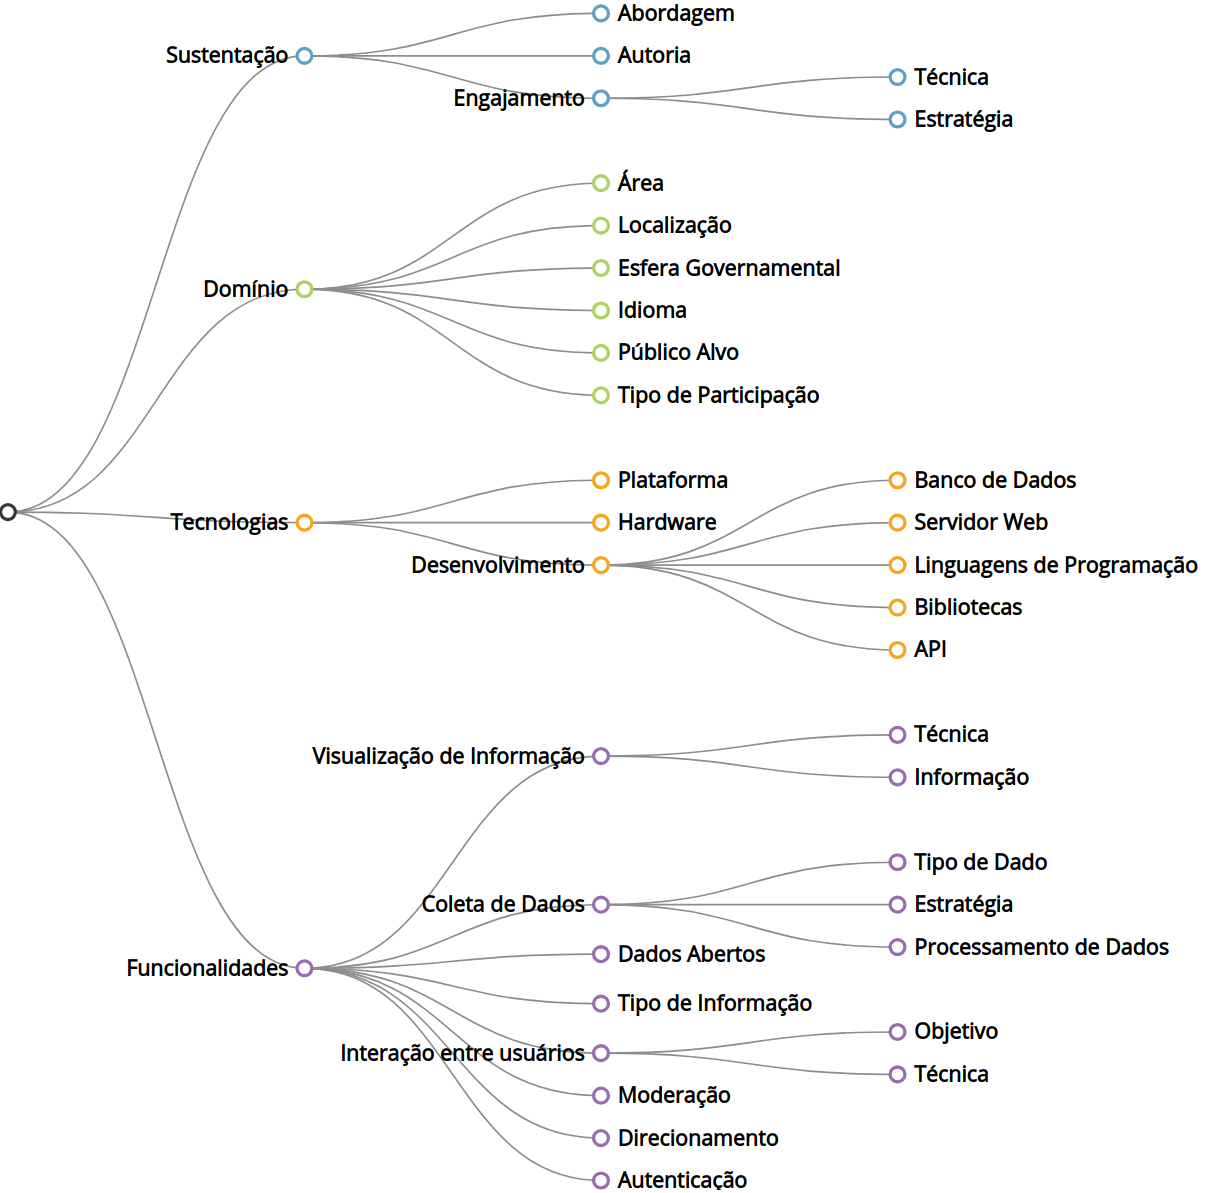
\includegraphics[scale=0.20]{./figuras/taxonopart-horizontal.png}
    \caption{e-TAPE Árvore}
    \label{fig:e-tapeArvore}
\end{figure}
\newpage

\par
Caso queira visualizar uma ferramenta já classificada, o usuário deve utilizar o campo de pesquisa, no canto superior esquerdo da tela Taxonomia.
Conforme o usuário for digitando o nome da ferramenta, o campo sugere ferramentas pelo modo de preenchimento automático. Se o usuário escreveu o nome da ferramenta corretamente 
e a ferramenta já estiver classificada, o usuário pode visualizar uma tabela com a classificação da 
ferramenta, vide Figura \ref{fig:show-ferramenta}.

\vspace{0.5cm}

\begin{figure}[!ht]
    \centering
    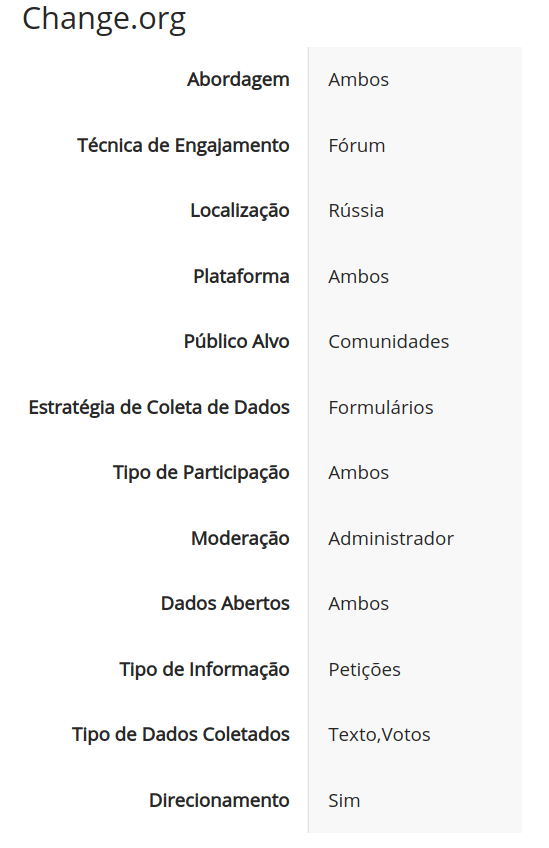
\includegraphics[scale=0.20]{./figuras/show-ferramenta.png}
    \caption{Visualizar ferramenta classificada}
    \label{fig:show-ferramenta}
\end{figure}


\par
Para classificar uma nova ferramenta, o usuário deve clicar no botão com o  sinal de "+", no canto inferior da tela Taxonomia, ilustrada na Figura \ref{fig:pag-taxonomia}. 
Tendo feito isso, o formulário para classificação da ferramenta é exibido, conforme ilustrado na Figura \ref{fig:new-ferramenta}. 

\begin{figure}[!ht]
    \centering
    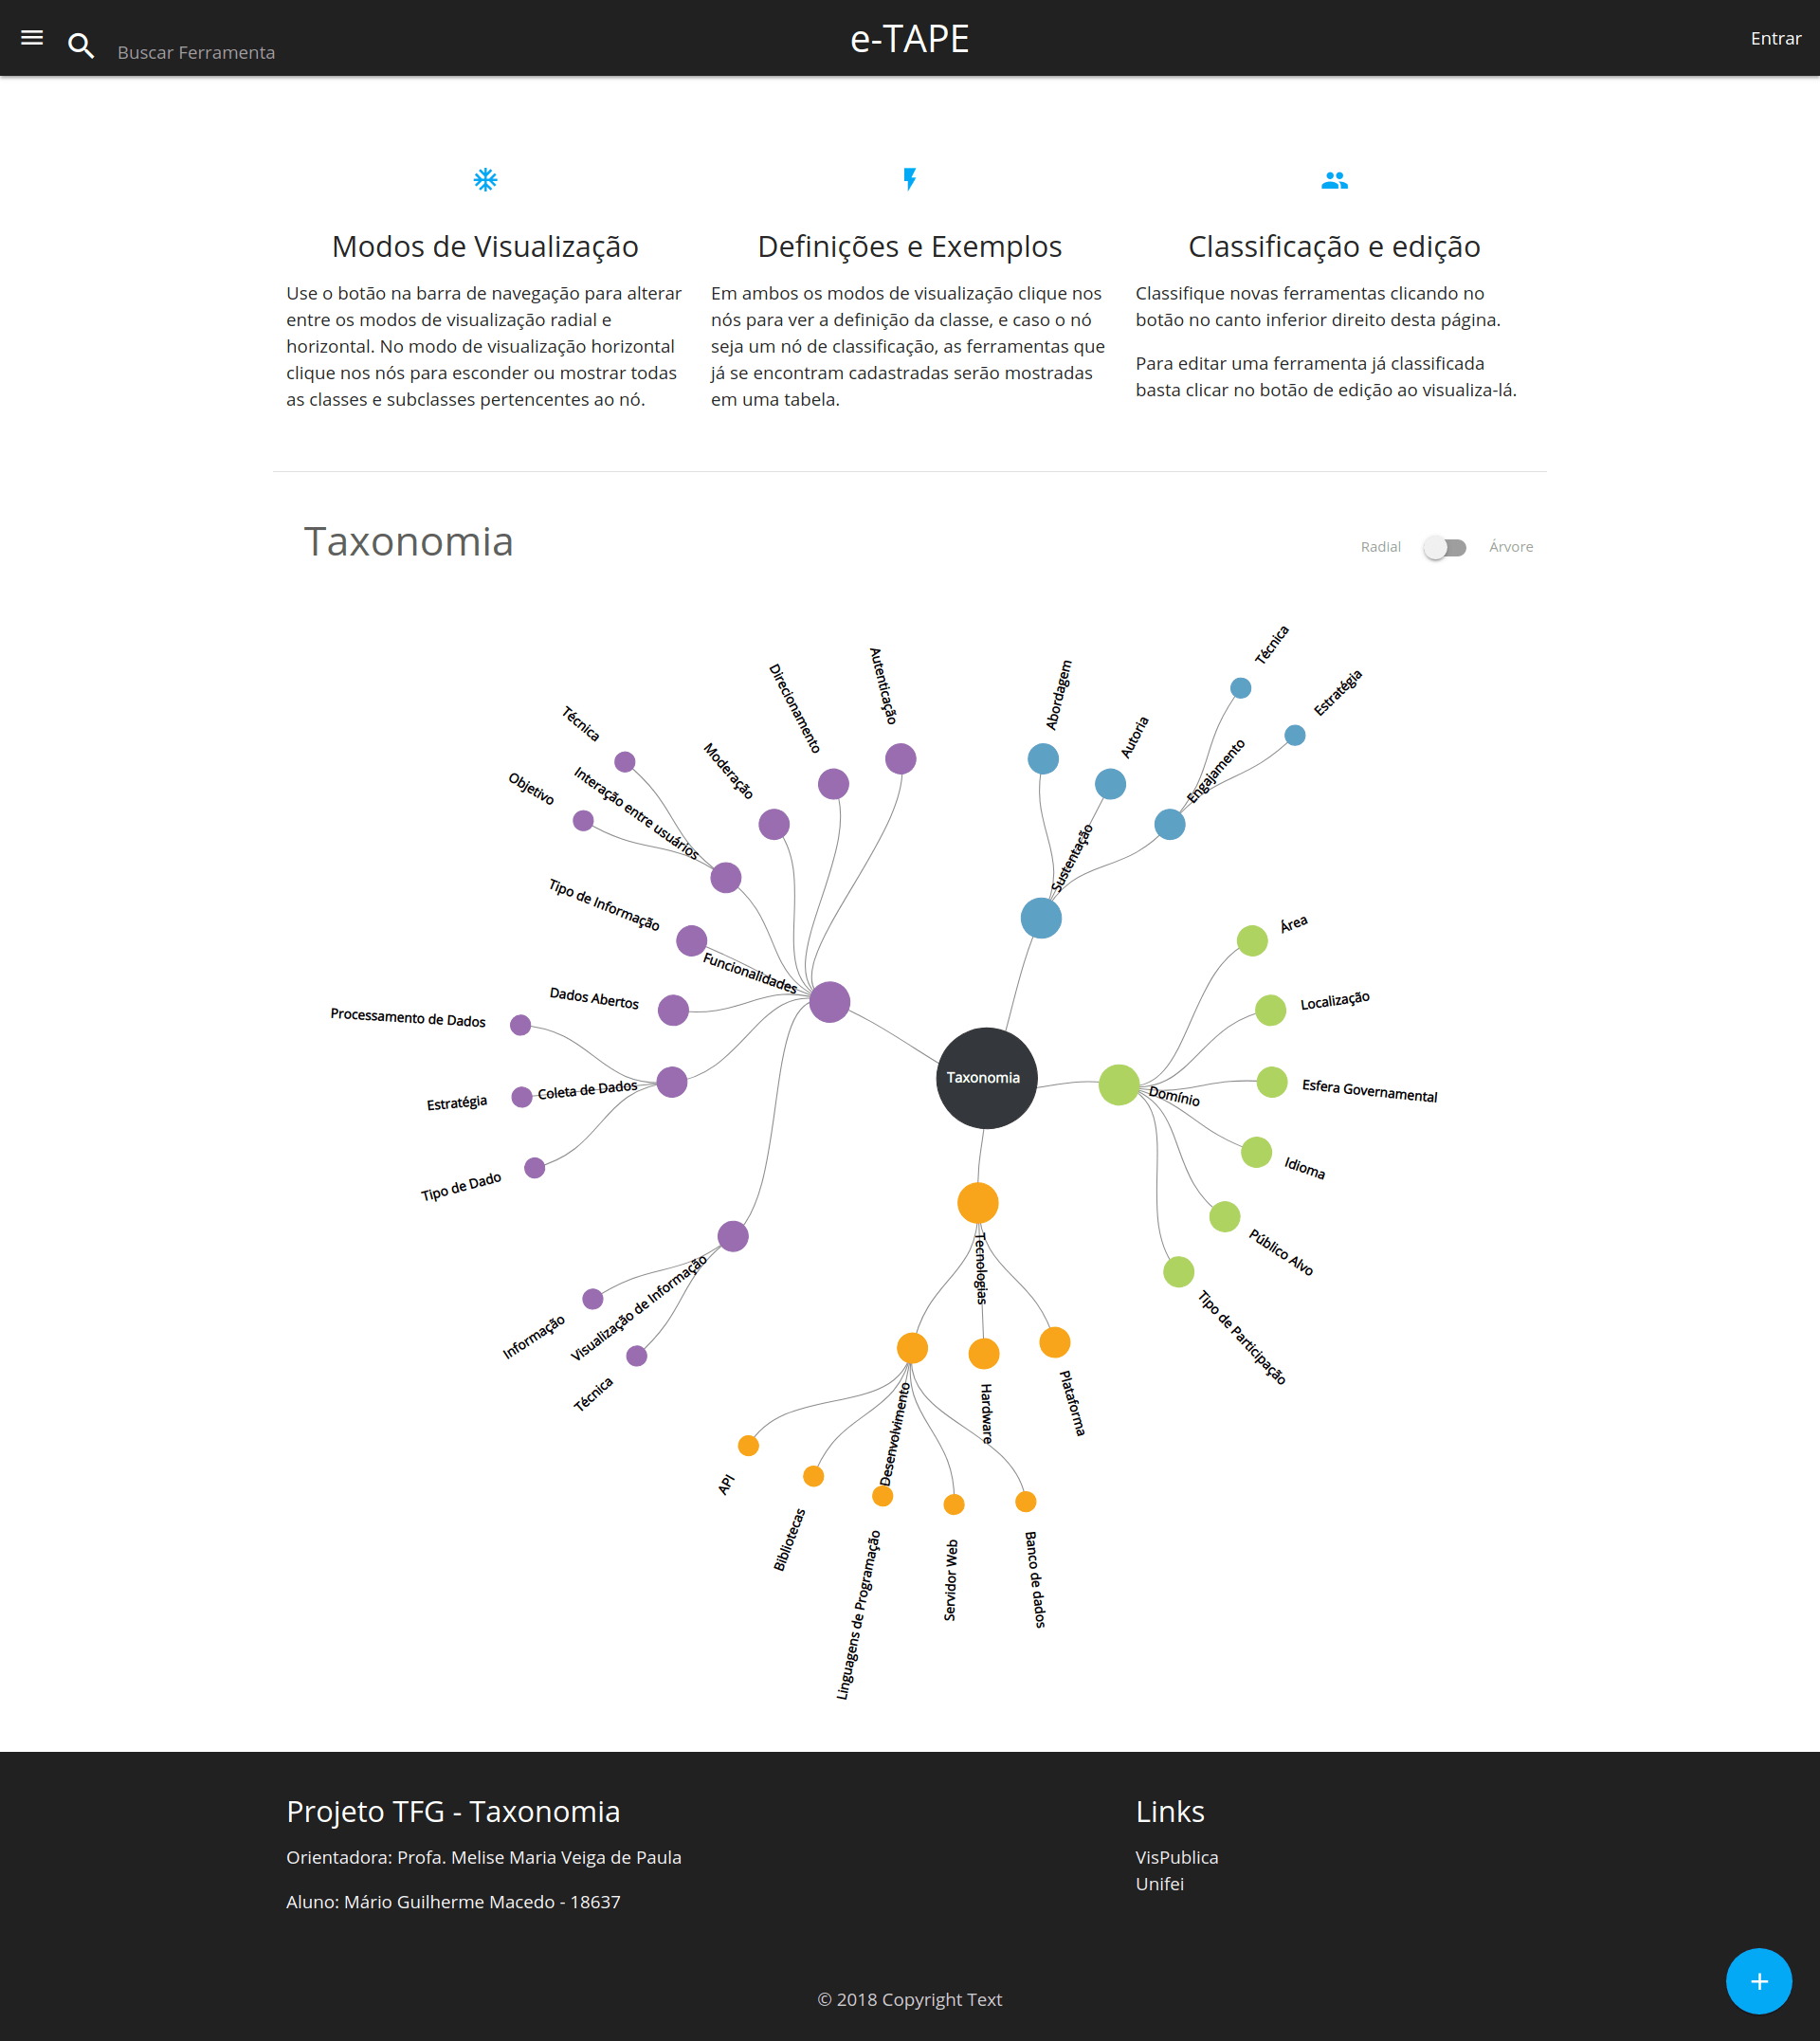
\includegraphics[scale=0.15]{./figuras/pagina-taxonomia.png}
    \caption{Página Taxonomia em e-TAPE }
    \label{fig:pag-taxonomia}
\end{figure}
\pagebreak

\begin{figure}[!ht]
    \centering
    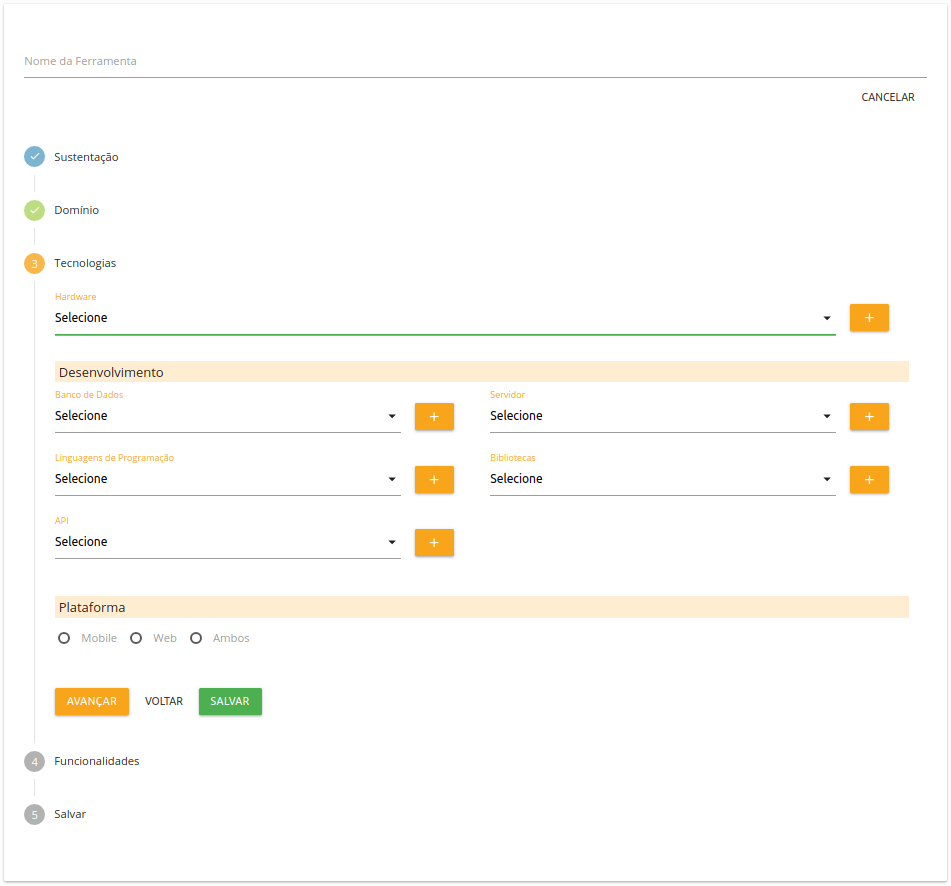
\includegraphics[scale=0.30]{./figuras/new-ferramenta.png}
    \caption{Formulário de classificação ferramentas}
    \label{fig:new-ferramenta}
\end{figure}


\par
O formulário de classificação de novas ferramentas foi dividido de acordo com os grupos definidos na TAPE (sustentação, domínio, tecnologias e funcionalidades), sendo o único campo de preenchimento obrigatório, o nome da ferramenta. Para finalizar a classificação da nova ferramenta o usuário pode, a qualquer momento, clicar no botão salvar. 
\par
Por se tratar de uma ferramenta colaborativa, o usuário visitante é capaz de visualizar e editar qualquer ferramenta já classificada por outros usuários. 
Para fazer isso, após visualizar a ferramenta, basta clicar no botão editar, que é representado pelo ícone de um lápis. 

\par
Caso o usuário visitante queria saber a definição de uma classe, duas opções estão disponíveis, parar o mouse em cima de algum nó da taxonomia, em qualquer modo de visualização, 
ou clicar no nó desejado. Para a primeira opção, é exibido um \textit{tooltip} com a definição do nó. Já para a segunda opção, é exibido um quadro com o nome da classe, descrição e 
uma lista com ferramentas classificadas e o valor ou as subclasses. A figura \ref{fig:tabela-ferramentas} demonstra essa segunda opção. 

\begin{figure}[!ht]
    \centering
    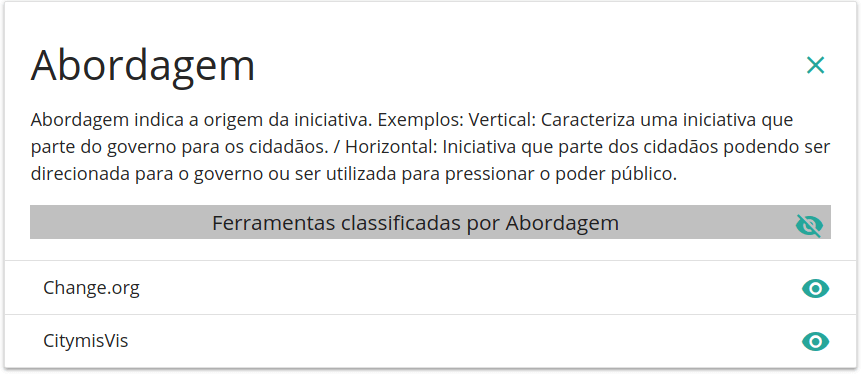
\includegraphics[scale=0.20]{./figuras/abordagem.png}
    \caption{Tabela com ferramentas classificadas segundo Abordagem}
    \label{fig:tabela-ferramentas}
\end{figure}
\par


A aplicação foi construída utilizando a plataforma de desenvolvimento Node.js. A escolha dessa plataforma justifica-se pelo conhecimento técnico da equipe
responsável pelo desenvolvimento da aplicação e pelo conceito fundamental da plataforma. Node.js é uma plataforma construída sobre o motor JavaScript do 
Google Chrome para desenvolver aplicações de rede escaláveis. Node.js usa um modelo de I/O direcionada a evento não bloqueante que o torna
apropriado para aplicações em tempo real com grande volume de troca de dados através de dispositivos distribuídos. 
\cite{nodejs}

\par
Após análise do modelo conceitual dos dados e das relações entre as entidades, foi identificada a necessidade da utilização de um banco de dados orientado a documentos para a 
persistência dos dados da aplicação. 
O \acrfull{sgbd} MongoDB foi escolhido por se tratar de uma ferramenta \textit{open source} e por permitir a integração com a plataforma Node.js 
\cite{mongodb}

\par
O \textit{front-end} da aplicação foi implementado com a utilização do \textit{framework} responsivo Materialize \cite{materialize}, pois esse mostrou-se uma opção adequada para o desenvolvimento da aplicação. Combinando o Materialize com o \textit{framework} de templates EJS \cite{ejs}, 
foi possível desenvolver a aplicação de maneira escalável e rápida. 


\par
Para a criação das visualizações da taxonomia, foram definidos dois modos de visualização, o modo radial, chamado na aplicação de e-TAPE 360º, e o modo horizontal, 
chamado de e-TAPE Árvore. Para a implementação de ambas visualizações, foi utilizada a biblioteca D3.js \cite{d3js}, uma biblioteca JavaScript para a manipulação de documentos 
baseada em dados que permite a visualização interativa de dados. 
O controle de versão da aplicação foi realizado através do sistema de controle de versão Git na plataforma GitLab, \cite{gitlab}.